\section{Spark}

\subsection{Présentation générale}

Spark est un framework open-source qui permet de traiter de larges volumes de données. C'est un framework qui est utilisé pour de grosse volumétries de données (supérieur en taille à 1 To de données). Pour des faibles volumétries de données, il existe différents outils plus simple et plus léger à mettre en place.

\subsection{Usages}

Spark permet de répondre à différents cas d'utilisations :

\begin{itemize}
  \item Faire de l'analyse de logs
  \item Traiter des fichiers de texte
  \item Faire de la recommandations pour des produits, des articles ...
  \item Faire de la détection de fraude et de la sécurité
  \item Recherche distribuée (Google, Facebook ...)
\end{itemize}

\subsection{Aspect fondamentale}

Spark tourne au seins d'un cluster  :

\begin{itemize}
  \item Spark peut fonctionner de différentes façon au niveau de la gestion du cluster. Il pourra être en standalone et ainsi se débrouiller de manière autonome, ou alors être géré par les gestionnaires de cluster YARN ou Mesos. Dans un cluster se basant sur Spark, on y trouvera un Master et plusieurs Workers. 
  Dans cette configuration le Master joue le rôle de répartiteur des différents traitements à effectuer entre les différents Workers. Par ailleurs, si l'on souhaite être tolérants aux pannes, le cluster doit disposer d'au moins deux Master, dont un en "standby" pour prévenir de son état en cas de perte du premier Master (ainsi, un autre Master Spark pourra être élu en Master principal). 
  Au fur et à mesure du traitement, le master principal fait des sauvegardes dans le second master pour que le Master en "standby" soit capable de prendre le relais.
  \item Spark permet de faire du traitement de manière distribué en répartissant le travail sur différents noeuds.
  \item Il se base sur un concept Hadoop qui est l'algorithme de MapReduce. C'est un modèle de programation pour traiter de fortes volumétries. Map Reduce possède plusieurs propriétés (équilibrage de charge, tolérance aux pannes, traitements distribués, traitements parallèles). Cela permet de découper la demande en plusieurs sous-problèmes.
  \item Spark offre également la possibilité de faire persister les données entre plusieurs machines ( les données sont stockées en mémoire et/ou sur disque).
\end{itemize}

\subsection{Resilient Distributed Dataset}

Les RDD sont au centre du framework Spark. Ils peuvent être vue comme des collections oû l'on y stocke des données. Ils possédent plusieurs propriétés :

\begin{itemize}
	\item Persistence : Les RDD peuvent être sur le disque et/ou sur la mémoire. Le fait de stocker les objects RDD en mémoire permet à Spark de réaliser des traitements plus rapide que ce que peut proposer Hadoop (Hadoop réalise uniquement des accès disque qui coûtent chers pour de grosse volumétrie).
	\item Résilience: Cela permet à Spark d'être tolérant aux pannes. Car dans un cluster les risques qu'un noeud tombe en panne et ne soit plus accessible est bien réaliste (probléme de réseau, de disque ....). De ce fait, Spark est capable de détecter qu'un noeud est encore en vie ou non. Ainsi, il sera capable de relancer les traitements de l'objet RDD qui ont échoué sur un autre noeud.
	\item Partitionnement : Au travers de Spark, on a la possibilité de découper les RDD en plusieurs parties. De ce fait, dans un RDD, les données vont être partitionnées. Soit Spark réalise le partionnement de manière arbitraire, soit on spécifie la taille des partitions désirée.
	\item Distribué : Comme les RDD sont partitionnés, on peut répartir le traitement sur plusieurs noeuds. Ainsi, cela permet à chaque noeud de travailler sur des tailles de données réduites et ainsi être capable de répondre le plus rapidement possible.
\end{itemize}

\subsection{Performances}

Pour montrer son efficacité au niveau du traitement des données, il est intéressant de savoir que Spark à battu le record de temps minimal précedemment détenu par Hadoop sur un tri distribué. Or, comme spécifié avant, les données sont en mémoire, ce qui permet aux traitements d'être réalisés jusqu'à 100 fois plus vite qu'avec Hadoop.

\ \\
Trie de 100 TB de données de maniéres distribué :
\ \\
\begin{itemize}
	\item Hadoop :
        \begin{itemize}
            \item Temps de calcul : 72 minutes
            \item Configuration : 2100 noeuds (50400 cores)
        \end{itemize}
	\item Spark :
		\begin{itemize}
        	\item Temps de calcul : 23 minutes
        	\item Configuration : 206 noeuds (6592 cores)
        \end{itemize}
\end{itemize}

\subsection{Utilisation dans le cadre du projet}
- Un job Spark, qui sera démarré par un orchestrateur Spark, va réaliser une sélection des musiques qui seront recommandées à un utilisateur cible d'une requête. Ce job récupère d'un filesystem basé sur HDFS un fichier résultat d'une requête: celle-ci va chercher les musiques aimées par d'autres personnes et qui ont également aimées au moins une musique de l'utilisateur cible.
- On parse les différentes données du fichier récupéré
- On utilise la fonction map des collections Spark pour sauvegarder en mémoire les noeuds et les arêtes que l'on va utiliser pour la création d'un graphe (sur lequel on effectuera nos algorithmes, voir partie la Graphx de la documentation).
- Une fois les traitements réalisés, on crée un fichier résultat contenant les "id" des titres recommandés pour l'utilisateur cible, et on l'envoie sur notre système de fichier HDFS.

\subsection{Infrastructure mise en place}
\ \\
\centerline{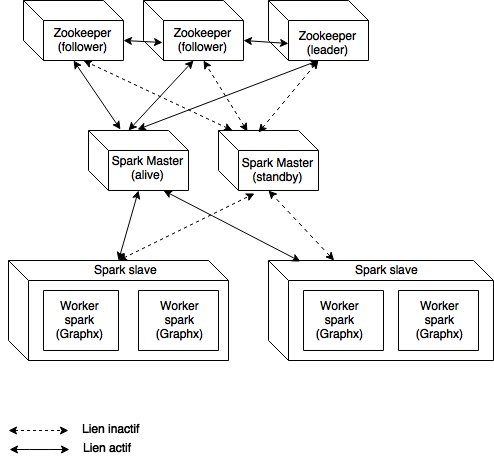
\includegraphics[scale=0.50]{pics/spark-infra.png}}
\centerline{\caption{Schéma globale de l'infrastructure mise en place pour SPARK}}
\ \\
\subsection{Haute disponibilité}
Pour permettre à notre cluster Spark d'être résilient, on va s'appuyer sur l'outil Zookeeper. Il va nous permettre d'élire un leader entre les deux Masters Spark. Ainsi, dans le cas où un leader meurt, Zookeeper se chargera de basculer sur le second Master Spark (en synchronisant le second Master selon l'état du premier). Cette opération de basculement entre les deux Masters peut prendre 1 à 2 minutes (le temps de détecter que le Master Spark est down et de mettre à jour l'état du second). 
Au niveau des workers, Spark gère lui-même l'aspect résilience de son cluster. Car comme cité plus haut, si un worker tombe, l'opération qui était en cours d'exécution dessus sera relancé sur un nouveau worker par l'intermédiaire du Master Spark.


